 %\documentclass[aps,prl,floatfix,12pt]{revtex4}
\documentclass[aps, pre, twocolumn, amsmath, superscriptaddress,showkeys,showpacs]{revtex4-1}
%\documentclass[aps,prb,floatfix,12pt]{revtex4}
%\documentclass[aps,preprint,floatfix]{revtex4}
%\documentclass[aps,12pt]{revtex4}
\usepackage{commath}
\usepackage[innercaption]{sidecap}
\usepackage{amssymb}
\usepackage{graphicx}% Include figure files
\usepackage{graphicx,epstopdf}
\usepackage{xcolor, soul}
\usepackage{dcolumn}% Align table columns on decimal point
\usepackage{bm}% bold math
\usepackage{mathrsfs} % script-like, curvy letters.
\usepackage{amsmath} %curvy letters.
\usepackage[colorlinks=true,linkcolor=blue,citecolor=blue]{hyperref}
%\usepackage[english]{babel}
\usepackage{fontenc}
\usepackage{float}
\usepackage{amsthm}
\usepackage{subfigure}
\usepackage{color}
\usepackage{ragged2e}
%\usepackage{bm}
%\usepackage{multirow}
\usepackage{enumerate}
%\usepackage{subcaption}
%\usepackage{ragged2e}
%\usepackage{subfigure}
\usepackage{hyperref}
%\usepackage[a4paper]{geometry}
%\geometry{top=1in,bottom=0.7in}
\topmargin=-.25in

\def\be{\begin{equation}}
	\def\ee{\end{equation}}
\def\bea{\begin{eqnarray}}
	\def\eea{\end{eqnarray}}
\def\bfg{\begin{figure}[H]}
	\def\efg{\end{figure}}



\begin{document}
	
%	\title{Diffusion induced revival of species in presence of natural death}
    \title{{\color{blue}Revival of species in the diffusive rock-paper-scissor dynamics in presence of natural death}}
	\author{Sahil Islam} 
	
	\email{thesahil.islam@gmail.com}
	
	\affiliation{Department of Physics, Jadavpur University, Jadavpur, Kolkata-700032}
	
	
	\author{Argha Mondal}
	\affiliation{School of Engineering, Amrita Vishwa Vidyapeetham, Amritapuri, Kollam 690525, India}
	\affiliation{Department of Mathematical Sciences, University of Essex, Wivenhoe Park, UK}
	\author{Sirshendu Bhattacharyya} 
	\thanks{Corresponding Author}
	\email{sirs.bh@gmail.com}
	
	\affiliation{Department of Physics, R.R.R Mahavidyalaya,
		Radhanagar, Hooghly 712406, India}
	
	\author{Chittaranjan Hens}
	\thanks{Corresponding Author}
	\email{chittaranjanhens@gmail.com}
	
	\affiliation{Physics and Applied Mathematics Unit, Indian Statistical Institute, Kolkata 700108, India}
	
	
	\begin{abstract}
		\noindent
		{\color{red}In the evolutionary dynamics of a rock-paper-scissor model, the effect of natural death plays an important role in deciding the fate of the system. Coexistence, being an unstable fixed point of the model, becomes very sensitive towards this parameter. In order to study the effect of mobility in such a system being explicitly dependent on mortality, we perform monte carlo simulation on a $2$-dimensional lattice having three cyclically-competing species. It is observed that high diffusivity of the system is capable of countering the effect of death to some extent. The spatio-temporal analysis has been performed and two site correlation has also been studied. Spatial distribution exhibits emergence of spiral patterns in presence of diffusion. It also shows that increasing diffusion can revive species close to extinction due to the effect of high death rate.}
		
	\end{abstract}	
	
	\maketitle
	
	\section{Introduction} 
	\label{intro}
	\noindent
	{\color{red}A stable ecosystem consists of different coexisting species with naturally balanced intra- and inter-species interactions like offspring production, predation-prey, intrinsic natural death etc. A natural goal of any ecological system is to maintain the biodiversity such that any species can avoid its extinction.} To capture {\color{red} the complexity in a stable ecological system, the principal idea behind evolutionary game dynamics that the survival or success of species depends on others is very useful \cite{szabo2007evolutionary,perc2017statistical,szolnoki2014cyclic,pennisi2005determines, mobilia2016influence,traulsen2006stochastic}.}
	%	1. Pennisi, E. What Determines Species Diversity? Science 2005, 309, 90.
	%	2. Hofbauer, J.; Sigmund, K. Evolutionary Games and Population Dynamics; Cambridge University Press:
	%	Cambridge, UK, 1998.
	%	3. Nowak, R.M. Evolutionary Dynamics; Belknap Press: Cambridge, MA, USA, 2006.
	%	4. Frey, E. Evolutionary game theory: Theoretical concepts and applications to microbial communities. Phys. A
	%	2010, 389, 4265–4298.
	%Games 2016, 7, 24 Mobilla 
	 A paradigmatic {\color{red}model of} evolutionary game dynamics such as the rock-paper-scissor (RPS) model, where  cyclic dominance \cite{arunachalam2020rock, kerr2002local, park2019fitness, reichenbach2007mobility, hashimoto2018clustering}  determines the fate of each strategy, {\color{red}often successfully mimics the emergence} of biodiversity in several natural systems. Colony formation and coexistence of several microbes \cite{ke2020effects, momeni2017lotka, kerr2002local,nahum2011evolution}, parasites \cite{cameron2009parasite, segura2013competition} etc. have been studied using this type of formalism. The stability of the {\it Uta stansburiana lizards} \cite{sinervo1996rock}, fermentation in the presence of oxygen and at high glucose concentrations \cite{pfeiffer2014evolutionary}  and diversity of coral-reef organisms \cite{jackson1975alleopathy} can  be explained with this type of cyclic game. 
	 {\color{red} The study of evolutionary RPS model can be characterized \cite{sinervo1996rock} in two formalisms: Lotka-Volterra (LV) approach \cite{bacaer2011lotka, lotka1920analytical, volterra1926fluctuations} in which particular species densities are conserved and May-Leonard (ML) approach \cite{chi1998asymmetric} where vacant sites are introduced and thereby species densities can be varied.}
	 %The coexistence and   extinction through interactions of these kind of species has been studied for a long time in both ecology \citep{tainaka2000physics}  and non linear science \citep{may1975nonlinear}. 
	 %These excitable systems are usually studied using some dynamical models like  
	 %
	 \par It has already been studied ({\color{red} both theoretically and experimentally}) that parameters such as system size, mobility, interaction region affect the stability and evolution of the system in a significant manner \cite{kerr2002local,pennisi2005determines,frey2010evolutionary,muller2010community}. In particular, demographic fluctuation breaks the coexistence leading to the extinction of certain species \cite{reichenbach2006coexistence,serrao2021rare,west2020fixation,berr2009zero}. Currently, {\color{red} the role of individual natural death (mortality) has been examined on the cyclic interaction of three species \cite{bhattacharyya2020mortality}.} It is observed that suitable intrinsic death rate of a species may dominate the effect of the birth or predation rates. As a result, a tiny change in the death rate may lead the system towards extinction or make any one species dominate over the others. 
	 %It has   been observed that static species forms colony in a two dimensional (2D) system to survive when hunting is  going on \cite{xxx}.  
	% {\color{red} In the absence of spatial degrees of freedom
	% 	and mutations, the presence of demographic fluctuations in finite populations leads to the loss of
	 %	biodiversity with the extinction of two species in a finite time, see, e.g., [11–16].}
	\par On the other hand, mobile species i.e., species having some kind of exchange or hopping probability may {\color{red} alter the erstwhile scenario of survival} \cite{kerr2002local,reichenbach2008self,kirkup2004antibiotic}. Depending on the strength of the mobility, several spatial structures such as spiral pattern \cite{ reichenbach2008self,avelino2012junctions, avelino2018directional} may emerge in the  extended 2D systems. In certain cases, these spirals grow in size depending on the rate of exchange and after a critical value of the hopping rate, the system shows anomalous behavior where only one species survives and other two go extinct. In particular, the size of spirals expands deliberately and it becomes larger than the system's size enabling any one of those species occupy the whole system \cite{reichenbach2007mobility}.
	\par In this backdrop, we revisit the effect of mobility in a cyclic RPS game dynamics where each species has its own intrinsic natural death rate.    
	Using Monte-Carlo simulations \cite{mooney1997monte, zio2013monte}, we have explored the effects of mobility in a 2D RPS system within ML formalism where {\color{red}each individual has a mortality rate i.e., all the species have a probability of death} irrespective of any other parameters like predation or reproduction. Interestingly, we have observed that for a {\color{red}high mortality rate, where the corresponding species was to vanish from the system, keeps up its existence for a certain strength of mobility}. {\color{blue} [Two or three more sentences are required here. The key observation, the critical $D$ where cross over occurs etc.]}
	\par {\color{red}The rest of the article is organized as follows. We describe the model, the dynamics and the method of simulation in Sec.~\ref{simulation}. The results are discussed in Sec.~\ref{results} and finally we conclude in Sec.~\ref{conclusion}.}
	\begin{figure*}[ht!]
	%\hspace*{-5mm}
	\centering
	\includegraphics[width=1.0\textwidth]{Diagram1.png}
	\caption{{\bf Schematic diagram of cyclic interaction and mobility in presence of natural death}. (a) Red arcs represent the cyclic predation between three species (red, blue, and green). Blue and blacks  arcs reflect the reproduction  and natural death respectively. (b) Mobility or exchange between two species or between vacant site and a randomly chosen species in lattice. The  lower lattice represents the changes of the position of the species due to migration/mobility (dashed ellipse). (c) and (e) In low death rate, the density of species remain finite for two mobility strength : smaller  $D=1\times 10^{-7}$  as well as in higher value $D=5\times 10^{-4}$. (d) In high death rate and in low diffusion, the density of each species is almost zero and no oscillatory behaviour is observed there. However  (e) In presence of higher diffusion, the oscillation with higher amplitude reemerges. In all the cases, $1000\times 1000$ lattice has been taken with unnormlaized predation and reproduction rates, $p=7$ and $r=7$ respectively for each of the species. {\color{blue}Here we have considered the low death rate $d=0$ and high death rate at $d=5$.}  }
	\label{fig1}
\end{figure*}	
	
	
	\section{The formulation of the Model and  Monte Carlo simulation}
	\label{simulation}
	
	\noindent
	We consider three species in a 2D lattice where each lattice site can either have one species or be vacant. In the beginning of the simulation, the species and vacancies are randomly oriented. Then we perform MC simulation {\color{red}governed by some interactions such as reproduction, predation, natural death and mobility all subjected to some predefined conditions}.
	\par {\color{red}We denote the three species by $A,\;B$ and $C$ and the corresponding densities by $\rho_a,\; \rho_b$ and $\rho_c$ respectively. The vacancies are denoted by $V$ and their density, by $\rho_v$ where $\rho_a + \rho_b + \rho_c + \rho_v = 1$. In the cyclic domination process, the predations can be represented by the following equations.}   
	\bea
	A + B & \longrightarrow & A + V \;\;\; \mbox{with rate}\;\; p_a\nonumber \\
	B + C & \longrightarrow & B + V \;\;\; \mbox{with rate}\;\; p_b\nonumber \\
	C + A & \longrightarrow & C + V \;\;\; \mbox{with rate}\;\; p_c
	\label{predation}
	\eea 
	{\color{red}where $p_{a,b,c}$ are the predation rates of $A,\;B$ and $C$ respectively. The reproductions can be expressed as}
   \bea
	A + V & \longrightarrow & A + A \;\;\; \mbox{with rate}\;\; r_a\nonumber \\
	B + V & \longrightarrow & B + B \;\;\; \mbox{with rate}\;\; r_b\nonumber \\
	C + V & \longrightarrow & C + C \;\;\; \mbox{with rate}\;\; r_c
	\label{reproduction}
	\eea
	{\color{red}The rate of reproductions are denoted by $r_{a,b,c}$. Alongside, the natural death of a species can make a site vacant as well.}
	\be
	S \longrightarrow  V \;\;\; \mbox{with rate}\;\; d_{a,b,c} 
	\label{death}
	\ee
	{\color{red}were $S$ represents any of the three species $A,\;B$ or $C$ and $V$ is the vacant site. The corresponding rate of death is $d_a,\;d_b$ or $d_c$. The cyclic predations, reproductions and deaths are schematically shown} in Fig.\ \ref{fig1}(a). Here red lizards (say, $A$) predate the greens ($B$), greens predate the blues ($C$) and blues predate the reds again. The blue arrows in Fig.\ \ref{fig1}(a) denote the birth of new species. Each lizard of  particular color creates another one of the same color (shown in smaller size). The black arrows indicate the natural death, and the grey lizards indicate the dead ones. Note that, we have considered identical predation, reproduction and death rate of each species: $p_a=p_b=p_c=p$, $r_a=r_b=r_c=r$ and $d_a=d_b=d_c=d$.	
		
  
Finally, we have considered that the species can exchange their positions with that of the neighboring species or vacancy governed by some probability:	
	\bea
	S + \phi(\neq S) & \longrightarrow & \phi(\neq S) + S \;\;\; \mbox{with rate}\;\; \epsilon
	\label{hop}
	\eea
Here $\phi$ can be either $A,\;B,\;C$ or $V$. Figure \ref{fig1}(b) describes this mobility process. {\color{blue}Here one green and one blue lizard in the upper lattice (marked by dotted ellipse)  exchanged their position and create a new lattice structure that is shown in the lower lattice of Fig.\ \ref{fig1}(b). In a similar way,  a lizard may hop to a vacant site (described as black filled dots). Note that, both swaps (between any two species or species vacant) do not happen simultaneously but in two different MC step}.      
We consider only nearest neighbour interactions and assume periodic boundary condition while doing the simulation. 
%i.e. if the lattice dimension is $N \times N$, then the $(N+1)^{th}$ site is the $1^{st}$ lattice site in both directions. 
The simulation starts with a random initial configration. At each MC step one lattice site is chosen randomly. {\color{red} Then another site is chosen out of the four nearest neighbors of the first site and possible operations (predation, reproduction, exchange) are made between the two sites with specified probabilities. Apart from this, the chosen first site is converted to a vacant one with the probability of death. All the probabilities are normalized by the rates $r,p,d$ and $ \epsilon$. This entire process is repeated until an equilibration is reached.} {\color{blue}Numerical simulations have been performed on lattice sizes $1000 \times 1000$ except for the extinction probability in higher diffusion calculation, where the lattice size is $500\time500$. Total number of MC steps required was from $10^4$ to $10^6$ depending on the lattice size and the rate of mobility.} 		
The exchange process in Eq.~(\ref{hop}) leads to an effective diffusion of the individual species governed by the macroscopic diffusion constant $D$. {\color{red} In our case of a 2-dimensional system, we connect this diffusion constant $D$ with the exchange rate $\epsilon$ through system size by the relation, $\epsilon=2 N^2 D $. \cite{reichenbach2007noise} }
%\par In each MC step the interactions occur with a probability normalized by the rates $r,p,d$ and $ \epsilon$ i.e. predation occurs with probability $p'\rightarrow p/(r+p+d+\epsilon)$, reproduction arises with probability $r' \rightarrow r/(r+p+d+\epsilon)$, natural death occurs with probability $d' \rightarrow d/(r+p+d+\epsilon)$, and the exchange process arises with probability $\epsilon' \rightarrow \epsilon/(r+p+d+\epsilon)$.\\
	
	\iffalse 
	The space-time dependence of the species densities can be expressed by these diffusion equations:
	
	\begin{eqnarray}
		\dfrac{\partial \rho_a(x,y,t)}{\partial t} &=& \rho_a(x,y,t)[r_a \rho_v(x,y,t) - p_c\rho_c(x,y,t) - d_a] \nonumber \\&&+ D \nabla^2 \rho_a(x,y,t) \nonumber\\[0.2cm]
		\dfrac{\partial \rho_b(x,y,t)}{\partial t} &=& \rho_b(x,y,t)[r_b \rho_v(x,y,t) - p_a\rho_a(x,y,t) - d_b] \nonumber \\&&+ D \nabla^2 \rho_b(x,y,t) \nonumber\\[0.2cm]
		\dfrac{\partial \rho_c(x,y,t)}{\partial t} &=& \rho_c(x,y,t)[r_c \rho_v(x,y,t) - p_b\rho_b(x,y,t) - d_c] \nonumber \\&&+ D \nabla^2 \rho_c(x,y,t)
		\label{rateeqn}
	\end{eqnarray}
	
	Here $\rho_v(x,y,t)=1-(\rho_a(x,y,t)+\rho_b(x,y,t)+\rho_c(x,y,t))$ the density of the vaccum.\\[0.2cm]
	And $\nabla^2 =\dfrac{\partial^2}{\partial x^2} + \dfrac{\partial^2}{\partial y^2} $ i.e. two-dimensional Laplacian operator. 

	
	\fi
	
		\begin{figure}
		%\hspace*{-5mm}
		\includegraphics[width=0.5\textwidth, height=4.5cm]{Diagram2.png}
		\caption{{\bf Role of diffusion and death rate on species coexistence.} (a) Total species densities are plotted against diffusion strength ($D$) for six constant death rates. We see that in lower death rates as the diffusion increases the total species density decreases slowly. At high death rate and low diffusion the species density is very low (gets extinct for $d=5$). But as the diffusion increases species density increases (revives even for $d=5$) and coexists. 
			(b) Total species density is plotted for two extreme diffusion constants ($ D=1.0\times 10^{7}$ and $ D=5.0\times 10^{-4}$ ) with increasing death rate. With increasing death rate, the total species density decreases. But the slope for these two cases are different. Lower diffusion leads to faster extinction but higher diffusion decreases the slope and leads to non-extinction of the species for a wider range of death rate.}
		\label{fig2-speciesdensity}
	\end{figure}
\section{Simulation results}
\label{results}
{\color{red} It has already been established \cite{bhattacharyya2020mortality} that the system has sharp dependence on natural death as compared to predation and reproduction. For a certain set of parameters {\color{blue}(condition?)} the system also exhibits coexistence of all the species resulting from an unstable fixed point having all non-zero densities. Now, with the incorporation of diffusion (or mobility) the fluctuation expectedly increases in the dynamics. However it does not jeopardize the coexistence in any case. Figure \ref{fig1}(c-f) reports the density of the species with respect to time for two different death rates and two different diffusion rates. Both for lower {\color{blue} (or no death?)} and higher death rate, the density of each species shows a stable oscillation. However the fluctuations are noted to be increased considerably when the diffusion rate increases from $1.0\times10^{-7}$ [Fig.~\ref{fig1}(c) \& (d)] to $5.0\times10^{-4}$ [Fig.~\ref{fig1}(e) \& (f)].}
% around an average value (approximately $0.3$ i.e $30\%$). 
%That means in lower death and diffusion, the entire system coexists with low vacant site. {\color{blue} 
%If we increase the diffusion of the species ($D=5.0\times10^{-4}$), we can observe that the fluctuation is higher compared to previous case and the mean density of each species oscillates around $0.26$. We have performed $10^5$ MC simulation to check whether the oscillations are stable or not.

\begin{figure*}
	%\hspace*{-5mm}
	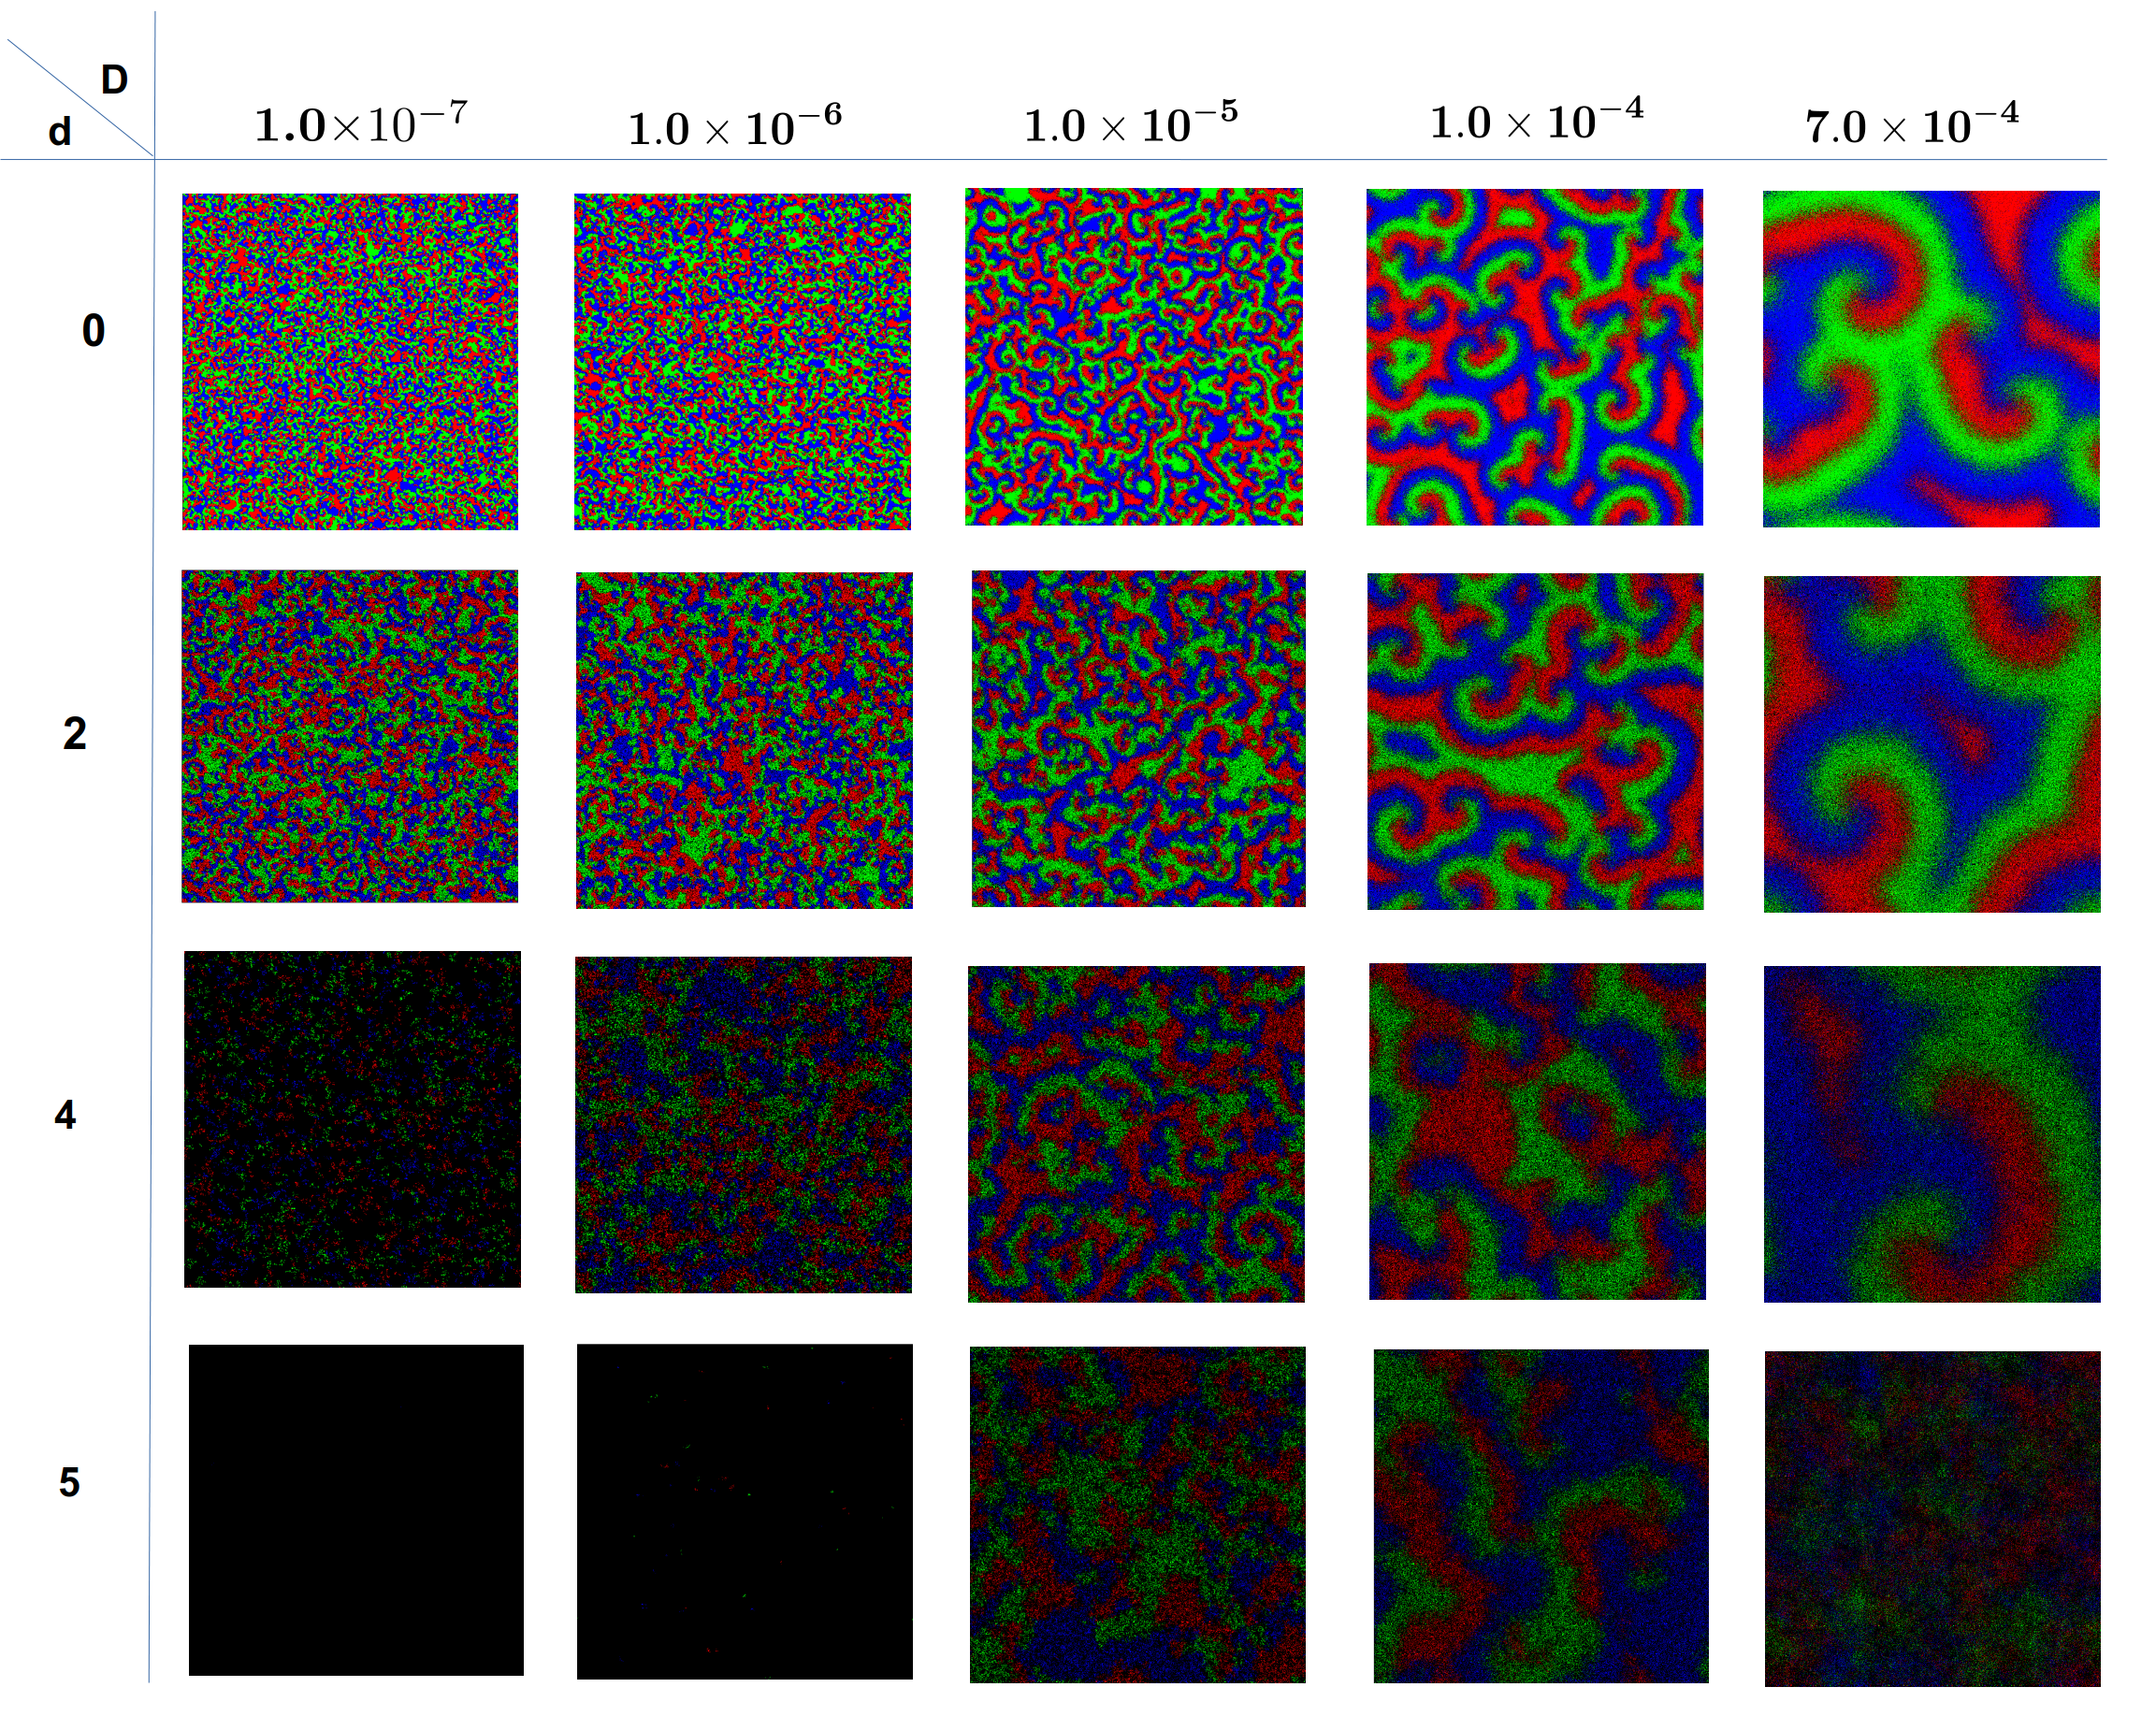
\includegraphics[width=16.9cm, height=13cm]{Diagram3.png}
	\caption{{\bf Spatial plot of species density for different death rate and diffusion strength.} Distribution of the species throughout the lattice is shown by colors : Red, Green and Blue for $A$, $B$, and $C$ respectively.  Black dots are  used for blank space. Diffusion strength is increased from $10^{-7}$ to $7\times 10^{-4}$ (from left to right). Natural death rate is increased from zero to $6$ (upper to bottom). }
	\label{fig3-spiral}
\end{figure*}
{\color{red} Increase of diffusion rate is seen to affect the average densities of the species significantly in the regime of high as well as low death rate. When death rate is high the average species densities remain very low leaving most of the lattice sites vacant for low diffusion (e.g see Fig.\ \ref{fig1}(d) for $d=4$). %If we increase the death further, all the species will die and the system will go extinct.
%However,  in this high death case if we increase the diffusion to higher value (i.e $5.0\time10^{-4}$, Fig.\ \ref{fig1}(f)), we observe that the oscillation revives and {\color{blue} this  oscillation is about a value higher than the low diffusion-high death case (here each of the species oscillates around $0.11$).
However, an increasing value of diffusion revives the species densities for the same rate of death. We can see in Fig.~\ref{fig1}(f) that the average denisity of the species has been raised as diffusion becomes $5.0\times10^{-4}$. The situation becomes opposite when we are in the low death regime. Incresing diffusion lowers the species densities there. This indicates that  the mobility of species outperforms the intrinsic death rate in these cases.} %and as a result the system can overcome extinction (number of vacant sites are decreased now) caused by natural death. 
This is our key observation and we explore this throughout the article. 

\par To delve deeper, we have calculated the {\color{red}total density of species ($1 - \rho_v$)} in the lattice as a function of diffusion strength for different death rates. {\color{red}The time-averaged total density is calculated following the definition
\be \rho_{\rm total} = \dfrac{1}{t_f - t_i}\sum\limits_{t_i}^{t_f} (\rho_a + \rho_b + \rho_c)\ee
where both $t_i$ and $t_f$ are in the equilibrated region of the MC simulation. Fig.\ \ref{fig2-speciesdensity}(a) shows the plots of $\rho_{\rm total}$ against diffusion rate for six different death rates.} At lower diffusion ($D\sim 10^{-7}$) and low death rates ($d=0$ and $d=1$ i.e., purple and green lines) {\color{red}the three species collectively occupy around $90\%$ and $80\%$ space of the whole lattice respectively. When the diffusion rate increases, $\rho_{\rm total}$ decreases continuously and saturates at certain values ($\sim 0.8$ for purple and $\sim 0.7$ for green line). The total density remains almost unaltered with varying diffusion for moderate death rates ($d\sim 2$). On the other hand, for species with higher death rates ($d\gtrsim 3$), an increase in $\rho_{\rm total}$ is observed with increasing diffusion rate. For very high death rate ($d\sim 5$), such revival of species occurs from a state almost close to extinction.} 
%But for death rates higher than this ($d=3,4,5$ i.e orange, yellow and blue lines) the phenomenon of decrease in species density gets reversed. {\color{blue} At low diffusion,  all the species become extinct (deep blue line, where death rate is $5$) or $~10\%$ species coexist (yellow line, death rate $4$). If we increase $D$, the total species density increases and finally saturates around $22\%$ for blue line or $39\%$ for yellow line. The  saturation appears at $d\sim 10^{-5}$. } 
In Figure  \ref{fig2-speciesdensity} (b), we have plotted the total species density as a function of  death rates for two extreme diffusion strengths: ($D=1.0\times10^{-7}$ and $D=5.0\times10^{-4}$). We see a linear decrease in total species density as we increase the death rates however, the slopes of these two lines are different. The lower diffusion rate (the magenta line) has a lower negative slope than the higher diffusion case (the green line). This leads to the fact that for higher diffusion rate the species density requires more higher death rate compared to the lower diffusion rate. Noticeably, due to the difference in slopes we observe an intersection of the two lines where the point of intersection occurs at a density $0.55$ or $55\%$. This intersection point gives a certain value of death rate and species density where two extreme diffusion rates leads to a similar state of the system. Thus both the figures support the fact that high diffusivity of a system can increase the coexistence probability by winning over the natural death rate. {\color{blue}[Mathematics possible for no diffusion? i.e., can we show the slope of $\rho_{total}$ vs $d$ for $D=0$ and establish anything? (see (4) in the notes below for details)]}
\\
For further analysis, we have plotted the species density spatially in a {\color{red} $XX\times XX$ lattice} (Fig.\  \ref{fig3-spiral}). {\color{red} Each of the figure is plotted at $t=10000$, a long time after equilibration.} In the first row where no natural death rate is considered, the size of the spirals increase from low diffusion to higher diffusion ($D=1.0\times 10^{-7}$ to $D=1\times 10^{-4}$ ). {\color{red}If we increase the diffusion rate further ($D\geq7.0\times 10^{-4}$), then the size of one spiral would be inflated so much that it would occupy the entire lattice leading to the situation of single species survival (not shown here).} %extinction of one of the species . 
This is consistent with the previously reported results \cite{reichenbach2007mobility}.   Now, if we introduce the natural death of each species, the size of the spirals grow more rapidly and {\color{red}one of the species becomes extinct around $D\sim XXX$ (second row, from left to right). In the third row, at death rate $d=4$} and at diffusion strength $D=1\times 10^{-7}$ a large fraction of the lattice sites become vacant. Thus a large collection of black dots appear in the spatial plot. However, if we increase $D$, the large spirals reappear in the lattice. Similar type of feature is observed for death rate $d=6$ as well. {\color{red}Thus, the diffusion has capability of diminishing the effect of death rate of the species. \st{We have ignored the mathematical analysis of such spiral patterns} \cite{ipsen2000amplitude,ipsen2000amplitudee,gong2003antispiral,mondal2019diffusion} \st{as we have just focused on the emergence of species in higher diffusion.}} \\
In order to investigate further, we have calculated the spatial correlation of the species. The correlation function is defined by:
	\begin{eqnarray}
g_{s_i s_j}(\mathbf{r}-\mathbf{r^\prime} , t) &\equiv& \langle s_i(\mathbf{r},t) s_j(\mathbf{r^\prime},t) \rangle -\langle s_i(\mathbf{r},t) \rangle  \langle  s_j(\mathbf{r^\prime},t) \rangle
\end{eqnarray}
\noindent
Here $s_{i,j}(\mathbf{r},t)$ ($i,j\in a,b,c$) represents the a species at the position $\mathbf{r}$ in the $2D$ lattice at a particular time $t$ \cite{reichenbach2007noise}. {\color{red}We study the correlation of species $A$ ($g_{s_a s_a}$) and it shows damped oscilaltion with respect to distance in case of the spiral patterns as observed in earlier studies \cite{reichenbach2007noise}.} The correlation length ($l_{\rm corr}$) is thereby determined by the length at which the correlation drops $1/e ^{th}$ of the maximum value \cite{reichenbach2008self}. {\color{red}All the plots shows that the correlation length increases with increasing diffusion indicating the size of a single patch in the spatial distribution getting bigger.} {\color{red}At lower diffusion, the correlation length for high death rate is almost nil mainly due to the extinction of species at that regime (Fig.\ \ref{fig4-corr}). At higher diffusion ($D\sim 10^{-5}$) the reemergence of species density (the blue and yellow line, also see the third and forth row of the Fig.\ \ref{fig3-spiral}) significantly boosts up the correlation length curve jointly with the inflated spiral size. %If we increase $D$ more, the size of the spiral is increased. The spirals grow more rapidly for higher death rate. 
Interestingly in the regime of high diffusion the growth of the correlation length, i.e. the size of the patch is elevated signifying that the species are prone to colony formation more when their mortality rates are high. This feature will be explored in more details in future.} {\color{blue}[Is it because larger death rate leads to single species survival?]}
%We will explore this interesting feature in near future.

	
	%\iffalse
%	It is naturally evident that the species should die more rapidly when their natural death rate increases. Increase in death rate makes the population of the species decrease and after a certain limit all the species dies making the system empty. But we have found that if we make the competetors mobile, then increasing the mobility can revive the coexistance of species.\\
%	From figure \ref{fig2} we see that for lower death rates increase in the diffusion leads to lower the total equilibrium density of the species. This happens upto a certain death rate . But after that for very high death rates, diffusion leads to increase the density.\\
%	\fi	
\section{conclusion}
\label{conclusion}	
	{\color{red} We study the role of diffusion in the spatio-temporal behavior of a 3-species ecosystem with cyclically dominating interaction. We also incorporate a rate of natural death which represent the finite lifetime of the living system. The ecosystem is mapped into a 2-dimensional lattice on which the RPS dynamics is studied in ML formalism through monte carlo simulation.
%We have explained the formulation and description of the model with parameters, various conditions for  the  numerical simulations that support the model equations. 
We mainly concentrate in the parameter region where the system exhibits coexistence. The natural death rate has already been proven to affect the coexistence significantly. Our present study reveal that high diffusion rate overshadows the act of natural death.} 
We have demonstrated how the time-averaged total density of the competing species changes with the rate of death as well as the rate of diffusion.
{\color{red}In addition, the study of two-site correlation length in the equilibrated spatial distribution shows that diffusion helps the species revive from the state of near-extinction in presence of very high death rate.}
% We have examined the change in correlation function and correlation length due to two interesting system parameters (). Higher values of diffusion can lead the system to extinction \cite{reichenbach2007mobility}. 
{\color{blue}We have reported the extinction probability and how the probability changes with increasing death rate. [plot?]}
{\color{red}The results therefore suggests that an ecosystem with its constituent species being highly mobile can evade possible extinction caused by increased mortality rate.}
%	It has been observed that mobility can dominate the effects of death and increase the species density in high death region where immobile species gets extinct. Death increases the correlation length upto a certain value however, in low mobility region the correlation length suddenly decreases due to the impact of natural death and with increasing mobility, the effect of death has been compromised and we obtain high value of correlation.
\par {\color{red}A diffusive system system allows inter-species exchange which eventually promotes colony formation among the species. However the influence of diffusion in the effect of death rate is counterintuitive because mobility and mortality, as incorporated in this system, are apparently two unconnected phenomena. Perhaps the formation of colonies resists the predation and thereby helps the species withstand possible extinction upto a limit. More investigation in this direction is in progress.} {\color{blue}[This paragraph should be written more clearly. Some future directios are to be added]}\\


	\begin{figure}
	%\hspace*{-5mm}
	\includegraphics[width=0.4\textwidth]{Diagram4.png}
	\caption{{\bf Various correlation  length at different death rate}. Correlation lengths (($l_{\rm corr}$)) are plotted against different diffusion strengths ($D$). In higher diffusion the length is enhanced. If the death rate is increased the length is also sharply increased. In intermediate diffusion strength ($D\sim 10^{-5}$), the species density revives fro higher death rate thus correlatuon becomes non zero (see the blue and yellow line). }
	\label{fig4-corr}
	\end{figure}
	\section{Acknowledgements} CH is supported by INSPIRE-Faculty grant (Code: IFA17-PH193). \\
	
	\section{References}
	\bibliography{bibliography_main}
	\bibliographystyle{apsrev4-1}
	
	{\color{blue} Additional notes from SB:\\
	1. Can you find some references (review or book) where monte carlo has been done in RPS system?\\
	2. Chop of the x-axis of Fig. 2(b) after d=4 so that the irregularity doesn't appear. \\
	3. Similarly chop off the end portion of the x-axis of Fig. 4 as well. \\
	4. From our previous paper, it can be shown that for coexistence, $\rho_{total}=-Md +C$, i.e., $\rho_{total}$ has a linear relationship with $d$ with $M$ and $C$ being constant for constant $p$ and $r$. \\
	Can we do similar derivation after inserting diffusion? Then Fig.2(b) can be explained mathematically. Moreover, it seems that the high diffusion plot may not be linear. \\
	5. Does two species survival occur for latge D? Or single species survival? \\
	6. In addition with using different colors for different plots, different symbols may also be used for convenience. \\
	7. Should we add the plot of the extinction probabilities? Because one line is written about it in the conclusion. \\
	8. Suggestions for Fig.1: (a) Make the arrows of same size so that the total figure looks perfectly cyclic. (b) Retain the upper diagram only and make the arrows straight for showing diffusion. Delete the big curly bracket and arrange the two arrows (low death and high death accordingly). (c and e) make y-scales equal and preferably put d=1 or 2 for showing low death (discussed before). (d and f) Can we make the y-scales equal here also?
	}
	
	
\end{document}
